\documentclass[a4paper,12pt]{extarticle}
\usepackage{geometry,microtype,mathtools,amsthm,amsmath,amsfonts,amssymb,marvosym,enumitem,hyperref}
\usepackage[table,xcdraw]{xcolor}
\usepackage[utf8]{inputenc}
\usepackage[font=small,labelfont=bf]{caption}
\setcounter{tocdepth}{1}
\theoremstyle{definition}
\newtheorem{definition}{Definition}
\newcommand{\myskip}{\par\null\par}
\renewcommand{\leq}{\leqslant}
\renewcommand{\geq}{\geqslant}
\newtheorem{theorem}{Theorem}
\newtheorem{corollary}{Corollary}[theorem]
\newtheorem*{remark}{Remark}
\newcommand{\R}{\mathbb{R}} \newcommand{\Q}{\mathbb{Q}} \newcommand{\Z}{\mathbb{Z}} \newcommand{\N}{\mathbb{N}}
\renewcommand\qedsymbol{QED}
\title{Math 431 Homework 3}
\author{Theo Koss}
\date{September 2022}
\begin{document}
\maketitle
\section*{Section 3.5}
\begin{itemize}
    \item \textbf{Problem 5:} Describe the symmetries of a square and prove that the set of symmetries is a group. Give a Cayley table for the symmetries. How many ways can the vertices of a square be permuted? Is each permutation necessarily a symmetry of the square? The symmetry group of the square is denoted by $D_4$.\begin{itemize}
    \item The symmetries of a square are as follows:\begin{itemize}
            \item The identity element, $e$.
            \item The 3 rotations, $r,r^2,r^3$. By $90^{\circ}$, $180^{\circ}$ and $270^{\circ}$ respectively.
            \item The 2 reflections, $t_x$ and $t_y$, horizontally and vertically.
            \item The 2 diagonal reflections, $t_{ac}$ and $t_{bd}$.
    \end{itemize} 8 elements in total.
    \item \begin{minipage}{\linewidth}
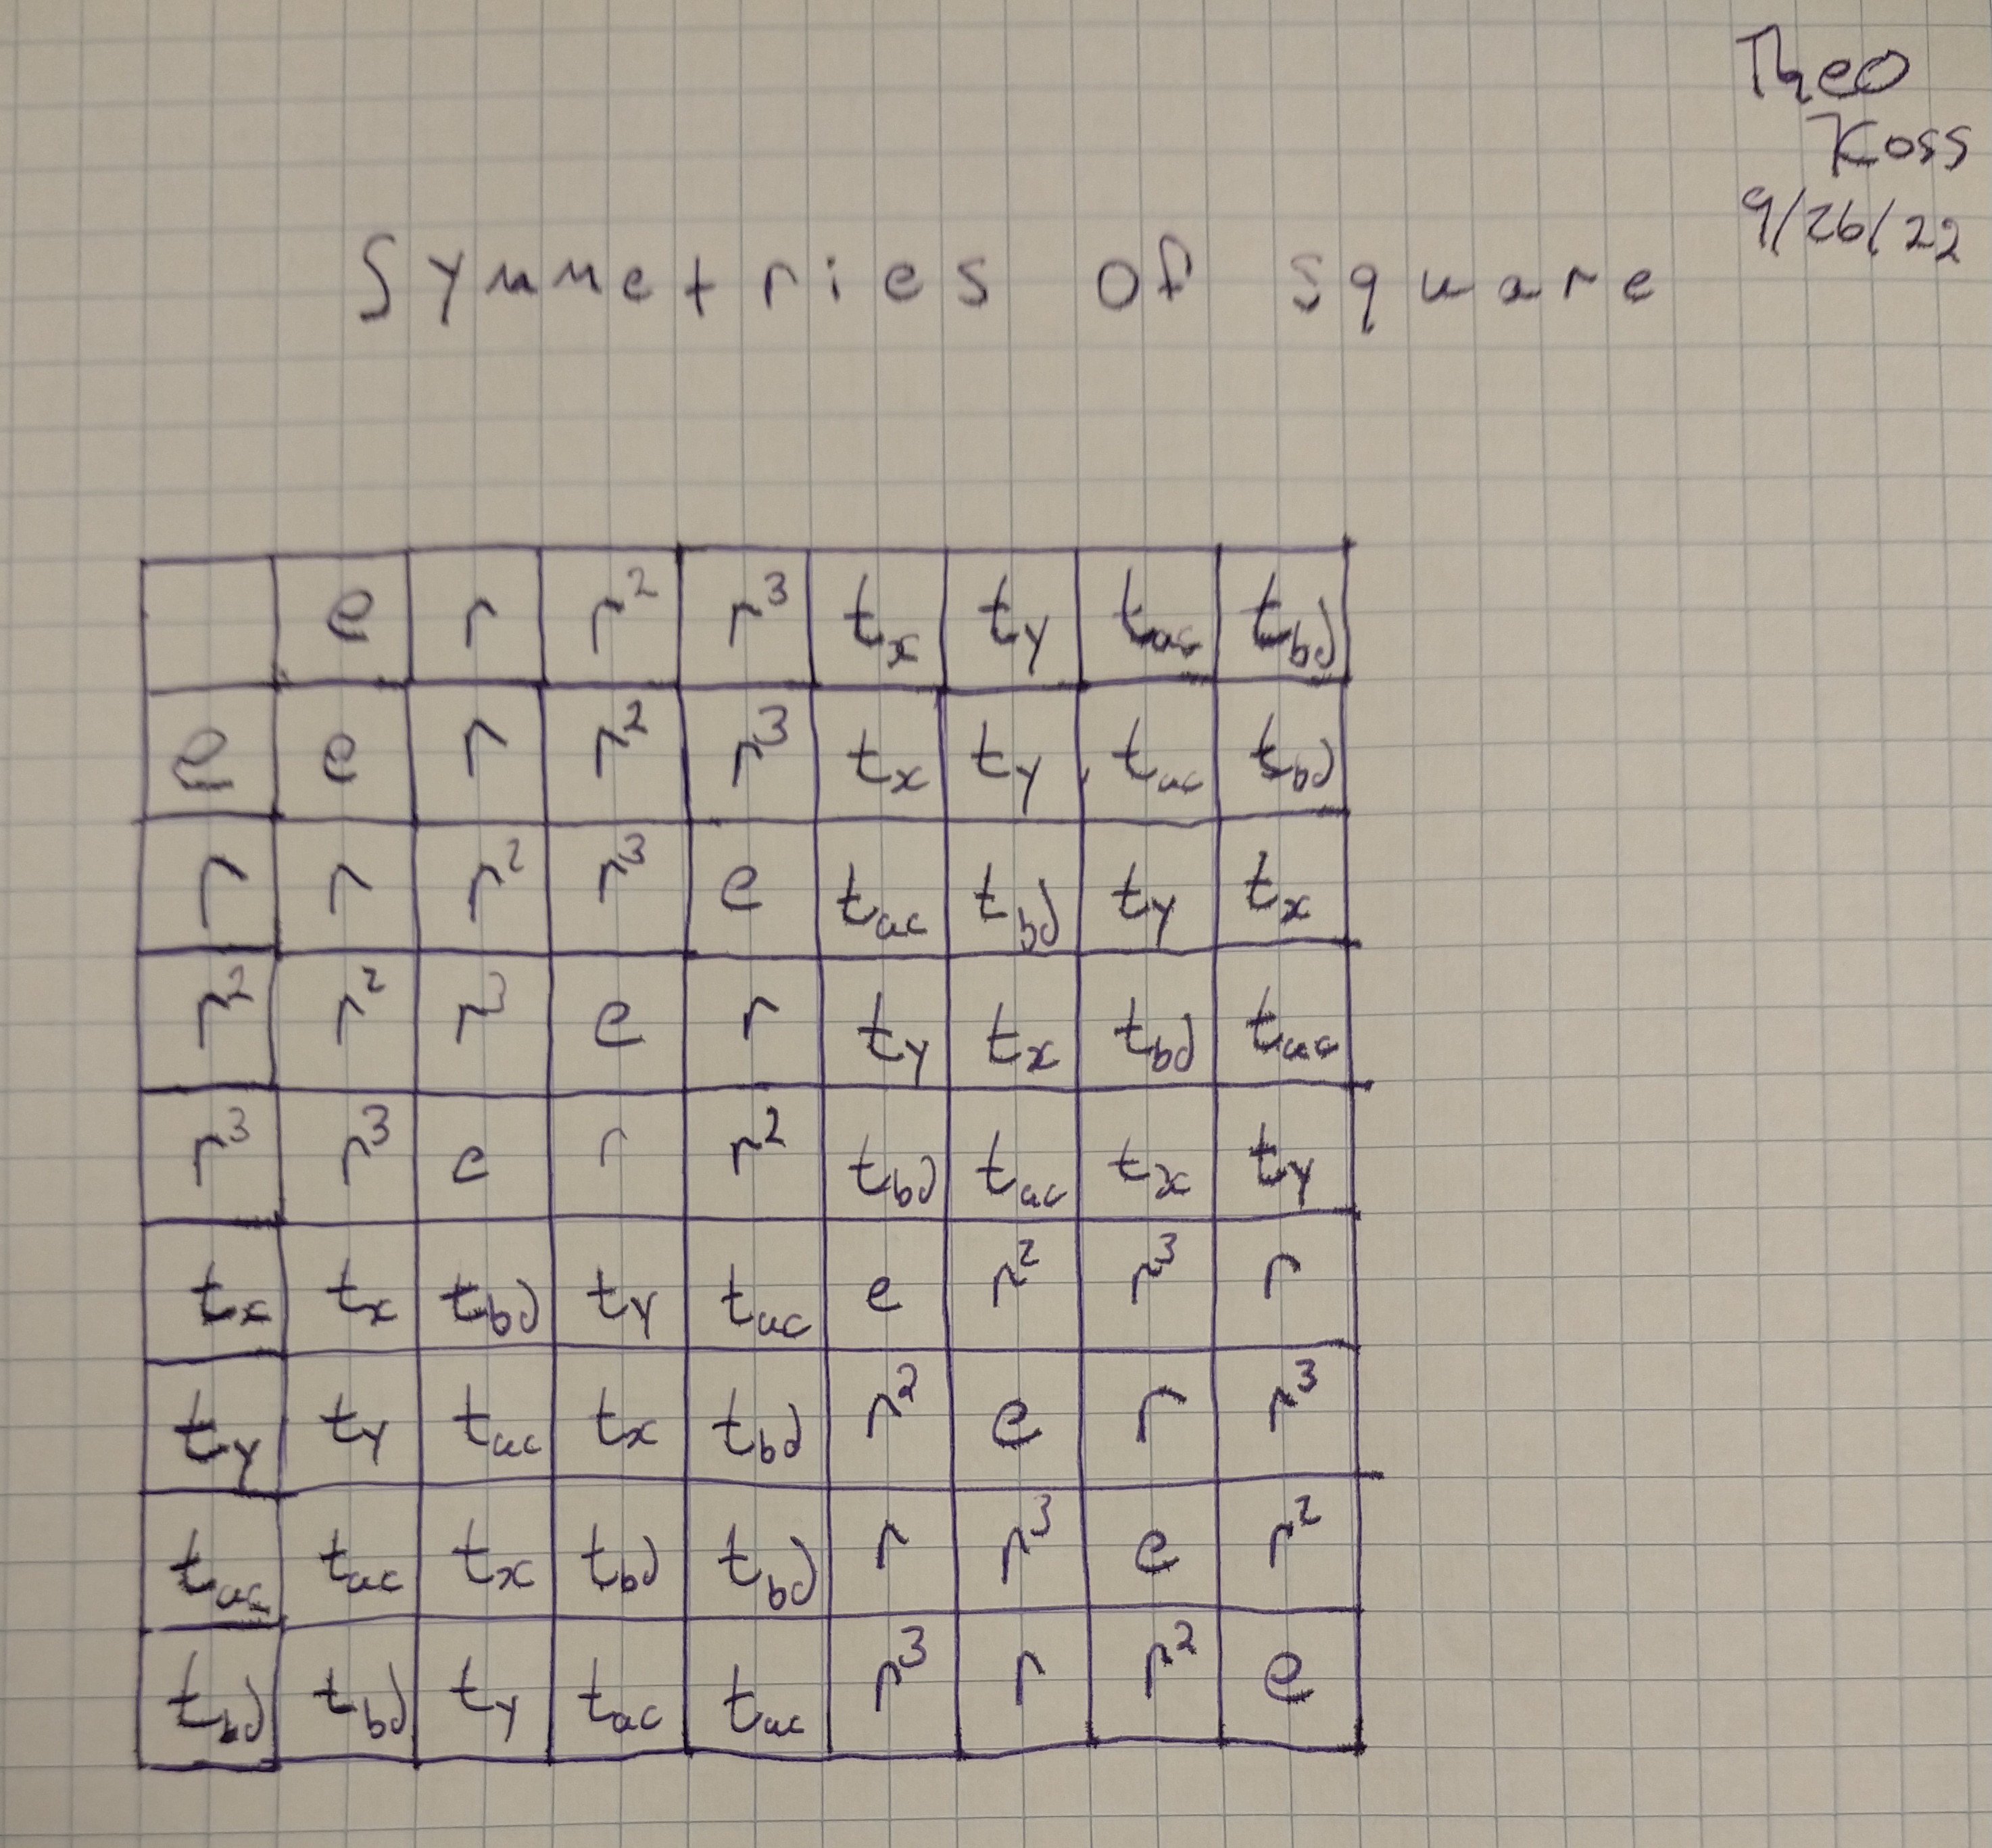
\includegraphics[width=\linewidth]{Photos/SymSquare.jpg}
\caption{figure}{\textbf{Figure 1:} Cayley table for symmetries of a square}\label{Fig1}
\end{minipage}%
\newpage
    \item \begin{proof}We must show the following for $D_4$ to be a group:\begin{enumerate}
        \item \textbf{Closure:} Using Figure 1, we can see that the set is closed.
        \item \textbf{Associativity:} As shown in class, function (or mapping) composition is \emph{always} associative.
        \item \textbf{Existence of Identity:} Again using Figure 1, we can see the element $e$ behaves as the identity element, $\forall a\in D_4,\  e\circ a=a\circ e=a$.
        \item \textbf{Existence of Inverses:} If each element has an inverse, \begin{align*}
            \forall a\in D_4,\exists a^{-1}\in D_4,\text{ s.t. } a\circ a^{-1}=a^{-1}\circ a=e
        \end{align*} then this is the same as saying there is one ``$e$'' in each row (or column) of our Cayley table. As we can tell simply by looking, there is one $e$ in each row of the Cayley table.
    \end{enumerate}Therefore, $D_4$ is a group.
    \end{proof}\textbf{Remark.} Perhaps notably, $D_4$ is not abelian.
    \item There are $4!=24$ ways to permute the vertices of a square. Not every permutation is a symmetry. For a square with vertices \{1,2,3,4\}. Consider \begin{align}\sigma=\left(\begin{array}{cccc}
1 & 2 & 3 & 4 \\
1 & 2 & 4 & 3
\end{array}\right)\end{align} for example. This is certainly a permutation of the vertices, however it is not a symmetry.
    \end{itemize}
    \item Problem 15: Prove or disprove that every group containing six elements is abelian.\begin{proof}Proof by counterexample, consider the group of the symmetries of an equilateral triangle, $D_3$. This has the following elements:\begin{itemize}
        \item Identity mapping, $e$.
        \item The 2 rotations, $r$ and $r^{-1}$, which denote rotations by $120^{\circ}$ clockwise and counterclockwise, respectively.
        \item The 3 reflections, $a,b$ and $c$, across the line going through each point (towards the middle).
    \end{itemize}
    $D_3$ has the Cayley table:\begin{align}\begin{array}{c|cccccc}\label{Tri}
      & e     & r     & r^{-1}   & a     & b   & c \\
\hline
e     & e     & r     & r^{-1}   & a     & b   & c \\
r     & r     & r^{-1}   & e     & b   & c & a     \\
r^{-1}   & r^{-1}   & e     & r     & c & a     & b   \\
a    & a     & c & b   & e     & r^{-1}   & r     \\
b   & a   & a     & c & r     & e     & r^{-1}   \\
c & c & b   & a     & r^{-1}   & r     & e     \\
\end{array}\end{align}It remains to show that this is a group, and that it is not abelian. Group:\begin{enumerate}
    \item \textbf{Closure:} Clearly from (\ref{Tri}), it is closed.
    \item \textbf{Associative:} Mapping composition is always associative.
    \item \textbf{Identity:} Again the element $e$ is the identity element. One can observe looking at the table that $\forall x\in D_3,\ x\circ e=e\circ x=x$.
    \item \textbf{Inverses:} Using the argument from above, we can see that each row has one $e$ in it, therefore each element has an inverse.
\end{enumerate}So $D_3$ is a group. Now consider $r\circ a=c$ this is clearly not equal to $a\circ r=b$. Therefore the group is not abelian.
    \end{proof}
\end{itemize}
\end{document}